\chapter{Contexte et cadre du projet}

\section{Introduction}

Ce premier chapitre présente une vue d'ensemble du stage en exposant l'entreprise d'accueil et le contexte du projet COTS. Il établit le cadre contextuel nécessaire à la compréhension des enjeux multidimensionnels de cette mission de fin d'études, centrée sur un défi d'ingénierie complexe : la conception et l'implémentation d'un framework d'automatisation des tests pour un système critique.

Cette mission s'articule autour d'un projet d'innovation technique majeur visant à transformer radicalement les processus d'assurance qualité du projet COTS par l'automatisation intelligente des tests de régression. Le défi principal consiste à concevoir une solution native pour une architecture microservices distribuée, intégrant les principes du Behavior-Driven Development (BDD) avec l'écosystème Spring Boot existant, tout en répondant aux exigences de fiabilité et de performance d'un système ferroviaire critique.

Au-delà des aspects purement techniques, cette expérience d'ingénieur nécessite une approche systémique intégrant plusieurs dimensions d'analyse complémentaires :

\textbf{La dimension technique et scientifique} explore les innovations méthodologiques apportées par l'hybridation BDD-microservices et évalue rigoureusement les performances de la solution développée, contribuant à l'enrichissement de l'état de l'art en automatisation de tests.

\textbf{La dimension organisationnelle} examine l'impact transformateur sur les pratiques de travail des équipes qualité, analysant les enjeux de conduite du changement et l'évolution des rôles professionnels induits par l'automatisation.

\textbf{La dimension environnementale et sociétale} évalue la contribution du projet à la durabilité numérique par l'optimisation des ressources informatiques et l'amélioration de la fiabilité du transport ferroviaire, infrastructure essentielle de la mobilité durable.

\textbf{La dimension stratégique et économique} analyse la création de valeur pour l'entreprise et le positionnement concurrentiel dans le secteur de la transformation numérique, ainsi que l'impact sur la modernisation du secteur ferroviaire français.

Cette présentation contextuelle constitue le socle indispensable pour appréhender l'analyse multidimensionnelle développée dans les chapitres suivants, illustrant la capacité d'un ingénieur à mener un projet d'innovation selon une approche rigoureuse et une vision systémique des enjeux contemporains de l'ingénierie logicielle.

\section{Sopra Steria : Acteur majeur de la transformation numérique}

\subsection{Présentation générale et positionnement stratégique}

Sopra Steria s'impose comme un acteur européen majeur de la transformation numérique, fort de plus de 50~000 collaborateurs répartis dans 30 pays et s'appuyant sur plus de 50 ans d'expérience. L'entreprise se distingue par sa capacité à combiner une compréhension approfondie des enjeux métiers avec une expertise technologique de pointe.

En tant que leader du conseil, des services numériques et du développement logiciel, Sopra Steria accompagne les plus grandes organisations dans leurs projets de transformation à travers plusieurs secteurs stratégiques :
\begin{itemize}
    \item Transport et mobilité
    \item Finance et banque  
    \item Secteur public et gouvernemental
    \item Industrie et énergie
\end{itemize}

\subsubsection{Indicateurs de performance}

Cette position de leadership se traduit par des indicateurs remarquables qui témoignent de la solidité et de la croissance de l'entreprise :

\begin{description}[leftmargin=3cm, labelwidth=2.5cm]
    \item[Chiffre d'affaires] Supérieur à 5 milliards d'euros, démontrant une performance financière solide et une croissance soutenue
    \item[Présence géographique] Dans 30 pays, soulignant sa portée internationale et sa capacité d'adaptation aux contextes locaux
    \item[Écosystème humain] Plus de 50~000 employés, reflétant des ressources substantielles et une diversité de compétences
    \item[Partenariats stratégiques] Avec les principaux fournisseurs technologiques et de solutions cloud du marché
    \item[Reconnaissance] Leader du conseil en transformation numérique par les grands analystes sectoriels
    \item[Portefeuille] Projets critiques réalisés avec succès pour les secteurs gouvernementaux et les grandes entreprises
\end{description}

\begin{figure}[H]
    \centering
    
\includegraphics[scale=0.8]{figures/sopra_presence_mondiale.png}
    \caption{Présence mondiale de Sopra Steria}
    \label{fig:sopra_presence}
\end{figure}

\subsubsection{Centre de Services de Nantes}

Le Centre de Services de Nantes représente un centre d'excellence spécialisé dans le domaine ferroviaire. Cette entité rassemble plus de 200 experts dédiés exclusivement aux projets SNCF, créant une concentration d'expertise qui permet une collaboration étroite avec les équipes du client. Les caractéristiques principales de ce centre incluent :
\begin{itemize}
    \item Un niveau de spécialisation technique et métier particulièrement élevé
    \item Une organisation en centres de compétences favorisant la mutualisation des connaissances
    \item Une approche managériale alliant leadership collaboratif et excellence technique
    \item Un environnement favorisant l'innovation tout en maintenant des standards de qualité rigoureux
\end{itemize}

\subsection{Mission, valeurs et approche différenciante}

\subsubsection{Mission stratégique}

La mission de Sopra Steria s'articule autour de l'accompagnement des organisations dans leur parcours de transformation numérique selon trois axes fondamentaux :

\begin{description}
    \item[Excellence Numérique] Conception et déploiement de solutions numériques innovantes qui maximisent la valeur métier et l'efficacité opérationnelle des clients, adaptées aux spécificités sectorielles et organisationnelles
    \item[Leadership Technologique] Positionnement à la pointe de l'innovation technologique tout en garantissant des solutions pragmatiques, évolutives et alignées sur les besoins métiers réels
    \item[Partenariats Stratégiques] Construction de relations durables fondées sur la confiance, l'expertise conseil et la capacité de livraison fiable de projets complexes à forte criticité
\end{description}

\subsubsection{Système de valeurs}

L'approche différenciante repose sur un système de valeurs profondément ancré qui guide l'ensemble des actions de l'entreprise :

\begin{description}
    \item[Orientation Client] Compréhension approfondie des enjeux clients et adaptation des solutions aux défis spécifiques de chaque organisation, garantissant une réponse sur mesure aux problématiques métiers
    \item[Excellence Technique] Maintien de standards élevés en développement logiciel, architecture système et innovation technologique, assurant la qualité et la pérennité des solutions déployées
    \item[Collaboration Intégrée] Promotion du travail d'équipe et du partage de connaissances, tant en interne qu'avec les équipes clients, pour maximiser l'efficacité collective et la réussite des projets
    \item[Amélioration Continue] Encouragement du développement professionnel permanent et de la veille technologique pour rester en phase avec l'évolution rapide des technologies et des pratiques sectorielles
\end{description}

\subsection{Contexte professionnel et environnement de mission}

Durant cette mission de stage, l'intégration s'est effectuée au sein de l'équipe projet COTS selon une organisation matricielle structurée, favorisant l'excellence technique et la collaboration interdisciplinaire nécessaires à la réussite du projet d'automatisation.

\subsubsection{Encadrement professionnel}
\begin{itemize}
    \item \textbf{Pierre Mirat} -- Chef de projet, supervision stratégique et coordination métier
    \item \textbf{Tom Richardson} -- Tech Lead expérimenté, encadrement technique et architectural
\end{itemize}

\subsubsection{Équipe collaborative}
\begin{itemize}
    \item \textbf{Louis Legendre} et \textbf{Mélina Loyant} -- Développeurs expérimentés, collaboration technique quotidienne
    \item \textbf{Florian Carré} et \textbf{Marie-Émilie Deschez} -- Analystes métier experts des processus SNCF, interface fonctionnelle essentielle
\end{itemize}

Cette organisation favorise l'acquisition d'une vision complète des enjeux techniques et métier, permettant de développer une approche d'ingénieur intégrant les contraintes organisationnelles et les exigences de qualité d'un système critique. L'environnement collaboratif et la nature interdisciplinaire du projet COTS offrent un cadre d'apprentissage optimal à l'intersection de l'ingénierie logicielle moderne, de l'expertise métier ferroviaire et de l'innovation en matière d'assurance qualité.

\section{Le projet COTS : Modernisation du système d'information ferroviaire}

\subsection{Vision stratégique et architecture fonctionnelle}

Le projet COTS (Catalogue des Offres de Transport et de Services) constitue une initiative stratégique majeure de modernisation du système d'information de la SNCF. Cette plateforme unifiée vise à remplacer l'écosystème actuel composé de multiples systèmes patrimoniaux disparates par un référentiel centralisé et cohérent, capable de gérer l'intégralité des offres de transport et services associés.

\subsubsection{Principes de conception}

L'architecture du système COTS repose sur des principes modernes garantissant une approche holistique de la gestion des données de transport :

\begin{description}
    \item[Centralisation Intelligente] Consolidation des données d'offres de transport provenant de sources multiples en un référentiel unique faisant autorité, éliminant définitivement les silos informationnels et les incohérences de données
    \item[Évolutivité Architecturale] Conception modulaire permettant la gestion de volumes de données croissants et de charges utilisateur variables tout en maintenant des performances optimales et une fiabilité constante
    \item[Intégration Systémique] Interconnexion harmonieuse avec l'ensemble des systèmes SNCF existants et les plateformes partenaires externes via des APIs RESTful et des protocoles de messaging asynchrones robustes
    \item[Réactivité Temps Réel] Support natif des mises à jour de données temps réel et implémentation d'une architecture événementielle garantissant une réactivité immédiate aux changements opérationnels
    \item[Maintenabilité Avancée] Utilisation de patterns architecturaux éprouvés et de technologies modernes assurant la durabilité à long terme, la facilité de maintenance et l'évolutivité fonctionnelle
    \item[Conformité Réglementaire] Respect strict des standards de l'industrie ferroviaire et des exigences réglementaires nationales et européennes en matière de sécurité, fiabilité et protection des données
\end{description}

\subsubsection{Technologies clés}

L'architecture microservices actuelle s'appuie sur une stack technologique moderne et éprouvée :
\begin{itemize}
    \item \textbf{Java Spring Boot} pour les services métiers et l'infrastructure applicative
    \item \textbf{MongoDB} pour la persistance documentaire et la gestion des données non-relationnelles
    \item \textbf{Apache Kafka} pour le streaming de données et la communication asynchrone inter-services
    \item \textbf{Architecture RESTful} pour les communications synchrones et l'exposition des APIs
\end{itemize}

\begin{figure}[H]
    \centering
    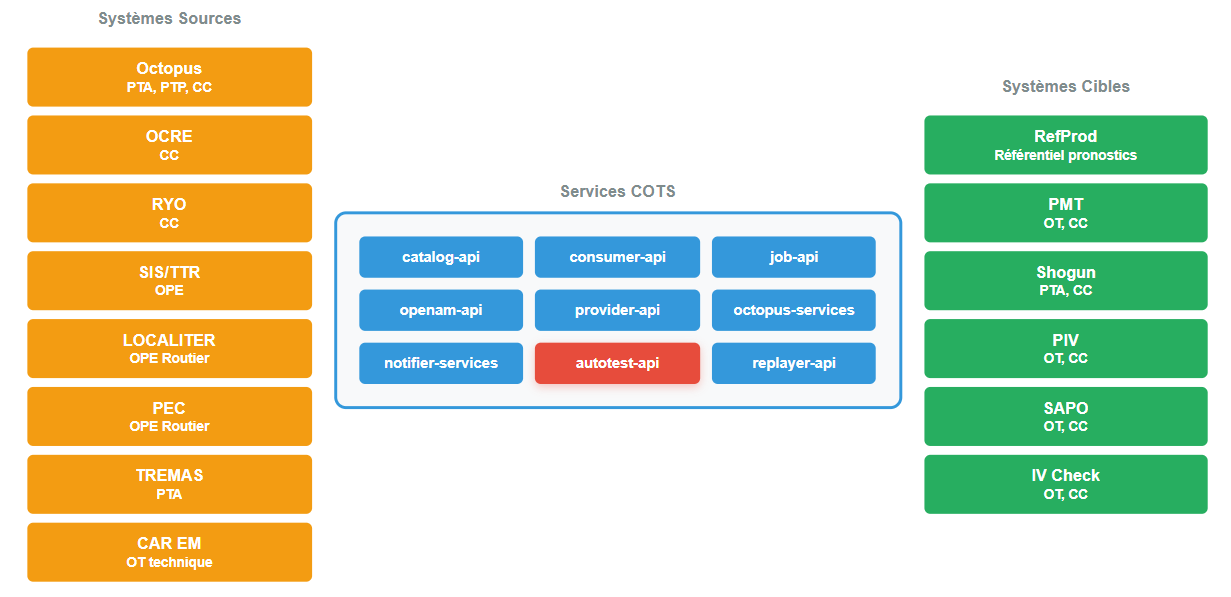
\includegraphics[scale=0.8]{figures/achitecture_cots.png}
    \caption{Architecture COTS - Microservices et Intégrations}
    \label{fig:architecture_cots}
\end{figure}

\subsection{Écosystème technique et services composants}

L'architecture microservices de COTS s'organise autour de neuf services critiques, chacun assumant des responsabilités spécifiques dans la chaîne de valeur du catalogue des offres :

\begin{description}
    \item[catalog-api] Service central de gestion des catalogues d'offres, responsable de la création, modification et orchestration du cycle de vie complet des offres de transport
    \item[consumer-api] Interface de consommation dédiée aux systèmes clients internes et externes, optimisant l'accès aux données du catalogue selon les profils utilisateurs
    \item[job-api] Orchestrateur de traitements batch et en temps réel, gérant l'exécution des processus métiers complexes et la synchronisation inter-systèmes
    \item[openam-api] Service d'authentification et d'autorisation sécurisée, intégrant les mécanismes de Single Sign-On et de gestion fine des droits d'accès
    \item[provider-api] Interface de fourniture de données vers les systèmes partenaires, assurant la diffusion contrôlée et sécurisée des informations catalogue
    \item[octopus-services] Ensemble de services métiers spécialisés, encapsulant la logique business complexe spécifique au domaine ferroviaire
    \item[notifier-services] Système de notification temps réel, gérant la diffusion d'événements et d'alertes vers les différents acteurs de l'écosystème
    \item[autotest-api] Service dédié à l'automatisation des tests, facilitant l'exécution de campagnes de validation et de non-régression
    \item[replayer-api] Système de rejeu de scénarios, permettant la reproduction et l'analyse de situations opérationnelles complexes
\end{description}

Cette architecture distribuée garantit une séparation claire des responsabilités, une scalabilité horizontale optimale, une maintenabilité simplifiée et la flexibilité nécessaire pour l'évolution future du système.

\subsection{Domaines d'application et valeur métier}

La polyvalence fonctionnelle du système COTS lui permet de couvrir l'ensemble des processus métiers liés à la gestion des offres de transport SNCF, créant une valeur ajoutée significative dans plusieurs domaines critiques.

\subsubsection{Gestion intégrée des offres de transport}
Le système centralise l'ensemble du cycle de vie des offres :
\begin{itemize}
    \item Création, modification et gestion du cycle de vie complet des offres de transport
    \item Couverture exhaustive des services SNCF (TGV, TER, Intercités, services régionaux)
    \item Processus harmonisés depuis la conception jusqu'au retrait des offres
    \item Gestion de la tarification et des conditions commerciales
\end{itemize}

\subsubsection{Optimisation économique et revenue management}
COTS supporte l'amélioration des performances financières par :
\begin{itemize}
    \item Support des stratégies de tarification dynamique et yield management
    \item Optimisation des revenus grâce à une vision unifiée et temps réel des données
    \item Analyse avancée de la demande client et ajustement proactif des offres
    \item Facilitation des études de marché et de la planification commerciale
\end{itemize}

\subsubsection{Excellence de l'expérience client}
L'amélioration de l'expérience utilisateur se traduit par :
\begin{itemize}
    \item Garantie d'une information d'offres cohérente, précise et actualisée en temps réel
    \item Harmonisation de l'information à travers l'ensemble des points de contact client
    \item Réduction des incohérences et des erreurs d'information
    \item Amélioration de la fiabilité du service d'information voyageur
\end{itemize}

\subsubsection{Écosystème partenarial étendu}
L'ouverture contrôlée vers l'écosystème externe facilite :
\begin{itemize}
    \item Les échanges de données harmonieux avec les partenaires commerciaux
    \item L'intégration avec les agences de voyage et distributeurs tiers
    \item Le support des systèmes de transport multimodaux et interopérables
    \item La facilitation des partenariats commerciaux stratégiques
\end{itemize}

\section{Enjeux et défis de la mission d'automatisation}

\subsection{Problématique complexe de l'assurance qualité}

Les projets logiciels d'envergure comme COTS évoluent dans un contexte où l'assurance qualité constitue un défi majeur, particulièrement critique dans le domaine ferroviaire où la fiabilité et la sécurité sont impératives. Cette problématique s'intensifie avec la complexité croissante des architectures distribuées modernes.

\subsubsection{Défis architecturaux des systèmes microservices}

La complexité intrinsèque des systèmes distribués génère des enjeux d'assurance qualité spécifiques :
\begin{itemize}
    \item Interdépendances complexes entre les neuf microservices de l'écosystème COTS
    \item Gestion de la cohérence des données distribuées et des transactions inter-services
    \item Validation end-to-end des parcours utilisateur dans un contexte distribué
    \item Maintien des performances et de la résilience sous charge variable
    \item Gestion des pannes en cascade et des mécanismes de récupération automatique
\end{itemize}

\subsubsection{Limitations critiques de l'approche manuelle}

L'approche actuelle de tests de non-régression (TNR), réalisée manuellement via l'outil ALM (Application Lifecycle Management), révèle des limitations structurelles majeures :

\begin{description}
    \item[Inefficience Temporelle Critique] Exécution séquentielle et manuelle générant des cycles de validation de 6 à 8 heures, incompatibles avec les objectifs de livraison continue et les contraintes opérationnelles d'un système critique
    \item[Vulnérabilité aux Erreurs Humaines] Manipulation manuelle des jeux de données complexes et paramétrage répétitif, introduisant un taux d'erreur estimé à 15-20\% dans les processus de validation
    \item[Saturation des Ressources Qualité] Mobilisation de 3 à 4 testeurs à temps plein sur des tâches répétitives, limitant drastiquement leur disponibilité pour l'innovation qualité et l'analyse exploratoire
    \item[Impact sur la Vélocité de Développement] Retards récurrents de 2 à 3 jours dans les cycles de déploiement, compromettant l'agilité requise par les enjeux métier
    \item[Déficit de Traçabilité et Reporting] Difficultés de consolidation des résultats et de génération de métriques fiables pour le pilotage qualité stratégique
\end{description}

\subsubsection{Enjeux spécifiques au contexte ferroviaire}

Le projet COTS fait face à des défis d'assurance qualité particuliers liés à son contexte d'application :
\begin{itemize}
    \item Validation des tests de régression suite aux mises à jour d'obsolescence technologique
    \item Assurance de la compatibilité inter-services lors des déploiements en production
    \item Maintien de la couverture de test exhaustive malgré l'augmentation de la complexité fonctionnelle
    \item Conformité aux standards de sécurité et de fiabilité du secteur ferroviaire
\end{itemize}

\subsection{Objectifs d'ingénierie et approche innovation}

Cette mission de stage s'articule autour d'un défi d'ingénierie majeur : concevoir et implémenter une solution d'automatisation révolutionnant les processus d'assurance qualité du projet COTS. L'approche adoptée vise à transformer une problématique opérationnelle en opportunité d'innovation technique et méthodologique.

\subsubsection{Objectifs techniques stratégiques}

La mission se structure autour de trois axes d'innovation complémentaires :

\begin{description}
    \item[Conception d'un Framework BDD Intégré] Développement d'une solution d'automatisation native basée sur Cucumber, intégrée organiquement à l'architecture Spring Boot existante, permettant l'expression des exigences métier en langage naturel tout en garantissant une exécution technique robuste
    \item[Orchestration CI/CD Intelligente] Implémentation d'un pipeline d'intégration continue sophistiqué avec Jenkins, intégrant des quality gates adaptatifs et des mécanismes de feedback automatique pour sécuriser les déploiements sans compromettre la vélocité de développement
    \item[Architecture de Tests Distribuée] Conception d'une infrastructure de test capable de valider efficacement les interactions complexes entre microservices, avec gestion automatisée des environnements et des données de test
\end{description}

\subsubsection{Innovation méthodologique et scientifique}

Le projet vise plusieurs contributions méthodologiques :
\begin{itemize}
    \item Développement d'une approche hybride BDD-microservices inédite dans le contexte ferroviaire
    \item Création de patterns de test réutilisables pour architectures distribuées critiques
    \item Élaboration de métriques de qualité avancées et de tableaux de bord prédictifs
    \item Contribution à l'état de l'art en automatisation de tests pour systèmes critiques
\end{itemize}

\subsubsection{Impacts opérationnels attendus}

Les bénéfices visés dépassent l'optimisation technique pour englober une transformation organisationnelle :
\begin{itemize}
    \item Réduction drastique des temps de cycles de validation (objectif : 85\% de réduction)
    \item Amélioration significative de la fiabilité des tests (objectif : 95\% de reproductibilité)
    \item Libération des ressources qualité pour des activités à forte valeur ajoutée
    \item Accélération des cycles de mise en production et amélioration de la réactivité métier
    \item Renforcement de la confiance dans les déploiements et réduction des risques opérationnels
\end{itemize}

\subsection{Méthodologie d'ingénierie et approche systémique}

La réalisation de cette mission s'appuie sur une méthodologie d'ingénierie rigoureuse, combinant approche agile et principes de conception architecturale, adaptée aux contraintes d'un système critique en production.

\subsubsection{Démarche de conception systémique}

L'approche méthodologique s'organise selon six phases intégrées :

\textbf{Phase 1 : Analyse Systémique et Spécification}
\begin{itemize}
    \item Analyse approfondie de l'architecture COTS et identification des points de fragilité qualité
    \item Étude des processus de test existants et cartographie des opportunités d'optimisation
    \item Spécification des exigences fonctionnelles et non-fonctionnelles du framework d'automatisation
    \item Définition des métriques de succès et des critères d'acceptation du projet
\end{itemize}

\textbf{Phase 2 : Conception Architecturale et Prototypage}
\begin{itemize}
    \item Conception de l'architecture du framework de tests avec patterns de résilience intégrés
    \item Prototypage rapide et validation des concepts techniques critiques
    \item Sélection et justification des choix technologiques (Cucumber, Spring Boot, Jenkins)
    \item Conception des interfaces et des mécanismes d'intégration avec l'écosystème existant
\end{itemize}

\textbf{Phase 3 : Développement Itératif et Validation Continue}
\begin{itemize}
    \item Implémentation incrémentale des composants du framework selon les principes TDD
    \item Développement des scénarios de test BDD en collaboration étroite avec les analystes métier
    \item Validation continue des performances et de la fiabilité en conditions quasi-production
    \item Optimisation progressive basée sur les retours d'expérience et les métriques collectées
\end{itemize}

\textbf{Phase 4 : Intégration et Orchestration}
\begin{itemize}
    \item Configuration des pipelines Jenkins avec quality gates intelligents et adaptatifs
    \item Intégration transparente dans les workflows de développement existants
    \item Mise en place des mécanismes de monitoring et d'alerting pour le suivi opérationnel
    \item Tests de charge et validation de la scalabilité du framework
\end{itemize}

\textbf{Phase 5 : Déploiement et Validation Opérationnelle}
\begin{itemize}
    \item Déploiement progressif en environnement de production avec stratégie de rollback
    \item Validation exhaustive des scénarios métier critiques en conditions réelles
    \item Collecte et analyse des métriques de performance et de fiabilité
    \item Ajustements finaux basés sur les retours opérationnels des équipes utilisatrices
\end{itemize}

\textbf{Phase 6 : Transfert de Connaissances et Pérennisation}
\begin{itemize}
    \item Élaboration d'une documentation technique et fonctionnelle complète
    \item Formation approfondie des équipes de développement et de qualité
    \item Définition des processus de maintenance et d'évolution du framework
    \item Capitalisation des bonnes pratiques et recommandations pour les projets futurs
\end{itemize}

\section{Résumé}

Ce chapitre contextuel a établi les fondements nécessaires à la compréhension de la mission de stage dans toute sa complexité technique et organisationnelle. L'analyse présentée structure la problématique selon trois dimensions d'analyse complémentaires qui préparent l'évaluation multidimensionnelle des chapitres suivants.

La présentation de Sopra Steria révèle l'environnement professionnel d'excellence dans lequel s'inscrit cette mission, soulignant l'expertise technique et la culture d'innovation de l'entreprise d'accueil. Le positionnement de leader européen de la transformation numérique contextualise la qualité des défis techniques proposés et l'ambition des solutions développées.

L'analyse détaillée du projet COTS démontre l'importance stratégique de cette initiative de modernisation pour la SNCF et révèle la complexité architecturale qui constitue le défi technique central de la mission. L'architecture microservices présentée illustre les enjeux contemporains de l'ingénierie logicielle et justifie l'innovation méthodologique nécessaire pour l'automatisation des tests.

La définition précise des enjeux et objectifs de la mission établit le cadre de référence pour l'évaluation des réalisations techniques et de leur impact opérationnel. Cette approche systémique permet d'appréhender l'articulation entre innovation technique, transformation organisationnelle et création de valeur, préparant l'analyse approfondie des dimensions technique, organisationnelle, environnementale et stratégique développées dans les chapitres suivants.

Cette mission illustre parfaitement les défis contemporains de l'ingénierie logicielle où la maîtrise technique doit s'accompagner d'une vision systémique des enjeux organisationnels et sociétaux pour créer des solutions durables et génératrices de valeur.